\documentclass[a4paper,11pt]{article}
\usepackage[dutch]{babel}
\usepackage{amsmath}
\usepackage{amssymb}
\usepackage{textcomp}
\usepackage{graphicx}
\usepackage[export]{adjustbox} 
\usepackage{siunitx}
\usepackage{parskip}
\usepackage{hyperref}
\usepackage{lipsum}
\usepackage[fixlanguage]{babelbib}
\usepackage{todonotes}
\usepackage{moreverb}
\usepackage{tabu}
\usepackage{mathtools}
\usepackage[font=small,format=plain,labelfont=bf,up,textfont=it,up]{caption}
\usepackage{multirow}
\usepackage{longtable}
\usepackage{listings}
\usepackage{tabularx}
\usepackage{url}
\usepackage{parskip}
\usepackage{pdfpages}
\usepackage{rotating}
\usepackage{enumitem}
\usepackage{a4wide}
\newcommand*{\bfrac}[2]{\genfrac{\lbrace}{\rbrace}{0pt}{}{#1}{#2}}
\everymath={\displaystyle}
\renewcommand{\figureautorefname}{Figuur}
\renewcommand{\tableautorefname}{Tabel}
\renewcommand{\partautorefname}{Deel}
\renewcommand{\appendixautorefname}{Appendix}
\renewcommand{\partautorefname}{Vergelijking}
\renewcommand{\Itemautorefname}{punt}
\renewcommand{\chapterautorefname}{Hoofdstuk}
\renewcommand{\sectionautorefname}{Sectie}
\renewcommand{\subsectionautorefname}{Sectie}
\renewcommand{\subsubsectionautorefname}{Sectie}
\renewcommand{\paragraphautorefname}{paragraaf}
\renewcommand{\Hfootnoteautorefname}{noot}
\renewcommand{\AMSautorefname}{Vergelijking}
\renewcommand{\theoremautorefname}{Stelling}
\renewcommand{\pageautorefname}{pagina}

% Symbolic alias stuff
\def\Ref#1{\hyperref[#1]{[#1]}}
\def\Section#1#2{\section[#1]{#1~\linebreak[3]
    \hfill{\texttt{\normalsize\Ref{#2}}}}\label{#2}}
\def\Item#1{\item[\texttt{\Ref{#1}}]\label{#1}\hfill\\}

\interfootnotelinepenalty=10000
\setlist[enumerate]{itemsep=0mm}

\begin{document}
\author{Randy Thiemann} 
\title{PDS \\ OpenMP Convolutie} 
\date{\today}
\maketitle

%%%%%%%%%%%%%%%%%%%%%%%%%%%%%%%%%%%%%%%%%%%%%%%%%%%%%%%%%%%%%%%%%%%%%%%%%%%%%%%%%
\section{Aanpak}
Ik heb voor de implementatie twee plaatsen gevonden om multi-threading toe te
passen. 

\begin{itemize}
    \item In de binnenste for loops waar de hadamar operatie van de afbeelding 
        en de kernel wordt uitgevoerd.
    \item In de buitenste for loops waar de convolutiefunctie wordt aangeroepen.
\end{itemize}

Voor het programma te testen op het VSC, heb ik beide methodes op mijn
persoonlijke computer getest. Hier uit is gebleken dat de eerste methode veel
minder effectief is dan de tweede methode, de eerste methode is 4 tot 5 keer 
trager afhankelijk van de scheduler, en dat als we deze combineren de code
zelfs trager draait dan zonder enige OpenMP optimizatie.

Ik heb dus besloten enkel de tweede methode toe te passen. Op mijn computer, met
een 7216x5412 afbeelding en een 31x31 kernel, duurt het gemiddeld 44 seconden op
zowel static, dynamic als guided scheduling.

%%%%%%%%%%%%%%%%%%%%%%%%%%%%%%%%%%%%%%%%%%%%%%%%%%%%%%%%%%%%%%%%%%%%%%%%%%%%%%%%%
\section{Resultaten}
Op het VSC heb ik met dezelfde afbeelding en kernel 10 runs gedaan met drie
verschillende schedulers: static, dynamic en guided. Deze test werd herhaald met 
1, 2, 4, 8, 16 en 20 cores. De gemiddelden en standaardafwijkingen zijn te
vinden in onderstaande grafieken.

\begin{figure}[h!]
    \centering
    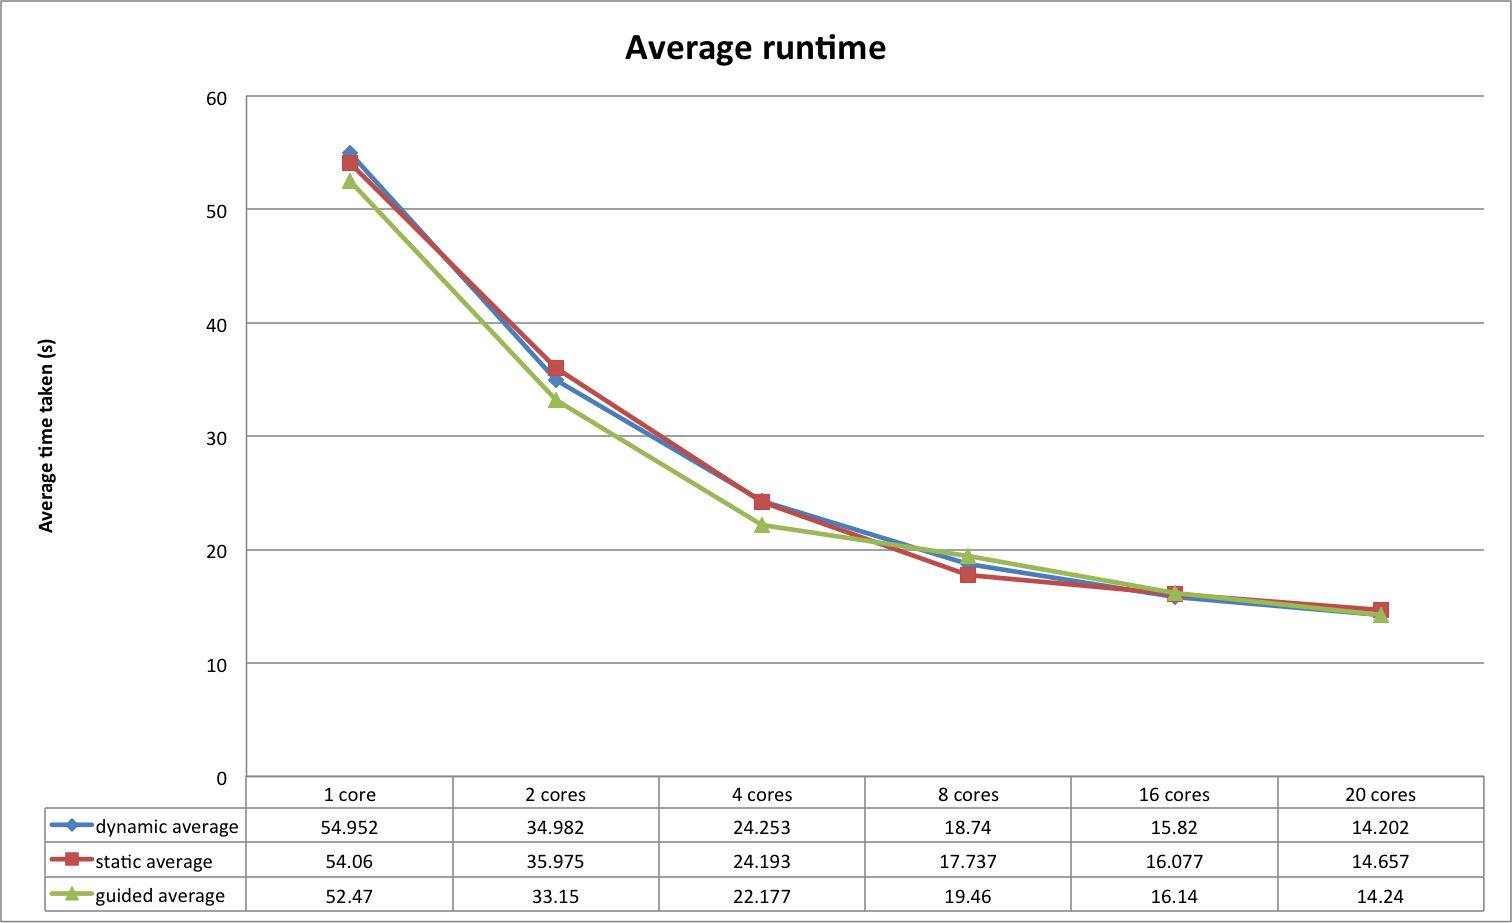
\includegraphics[width=\textwidth]{average}
\end{figure}

\begin{figure}[h!]
    \centering
    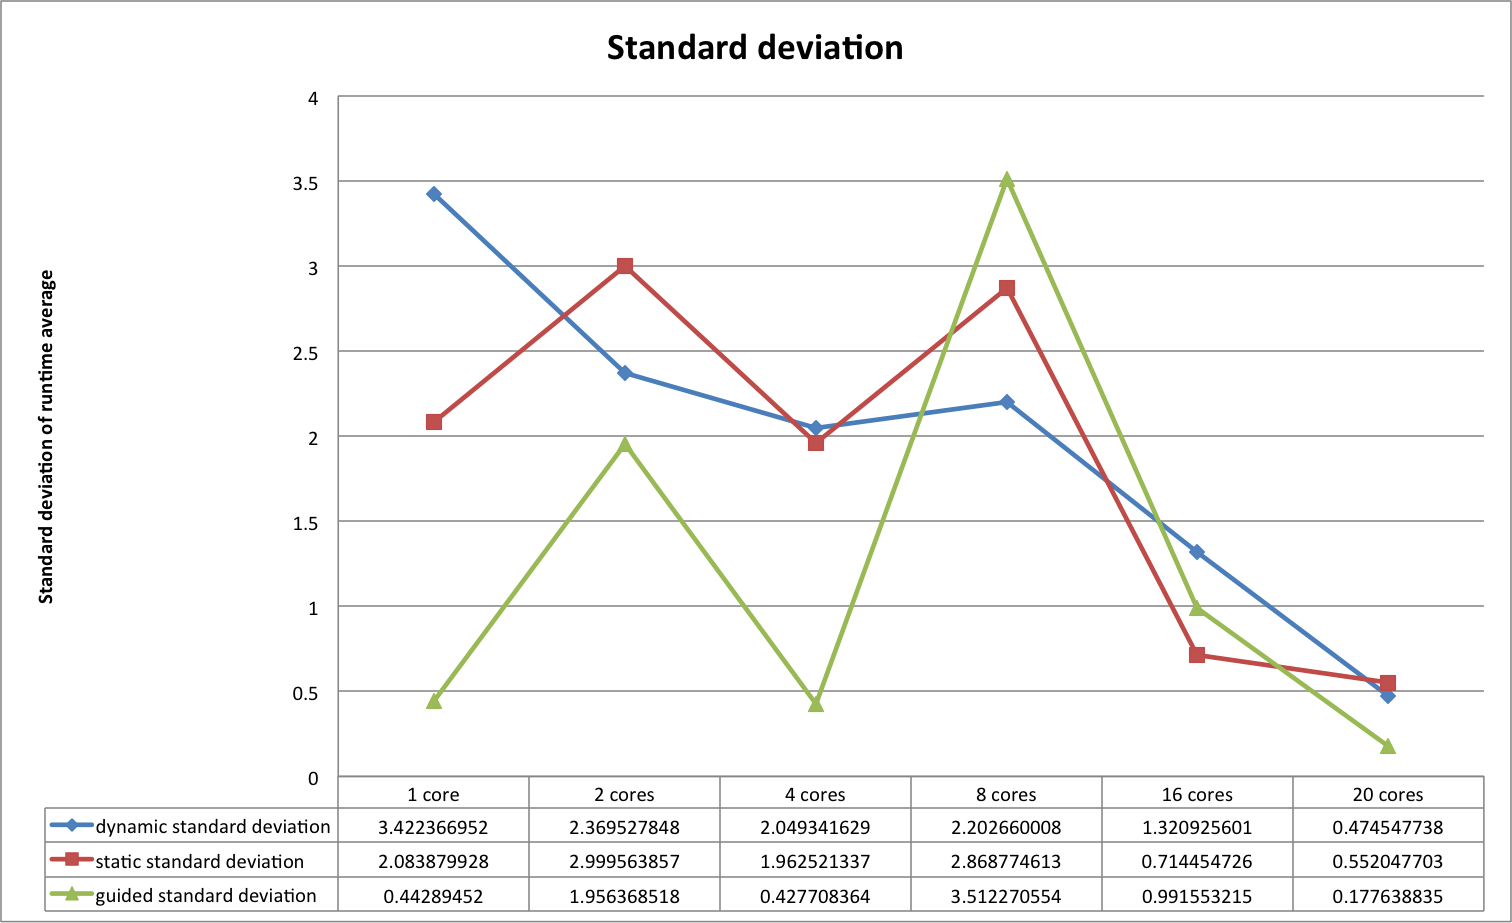
\includegraphics[width=\textwidth]{stdev}
\end{figure}

Hieruit blijkt dat tot 4 cores, op het vsc, guided de beste gemiddelde runtime
geeft. Dan is voor 8 en 16 cores static het beste, eindigend met dynamic op
20 cores. De algemene trend is wel zoals verwacht.

In de standaardafwijkingen is over het algemeen de methode met het laagste
gemiddelde ook deze met de laagste standaardafwijking.

\end{document}
